\documentclass[]{AVSSimReportMemo}
\usepackage{AVS}

\newcommand{\ModuleName}{velocityPoint}
\newcommand{\subject}{Guidance Module for Velocity Axis Pointing}
\newcommand{\status}{Initial Version}
\newcommand{\preparer}{M. Cols}
\newcommand{\summary}{Generate the attitude reference to perform a constant pointing towards a Velocity orbit axis}


\begin{document}

\makeCover


%
% enter the revision documentation here
% to add more lines, copy the table entry and the \hline, and paste after the current entry.
%
\pagestyle{empty}
{\renewcommand{\arraystretch}{2}
\noindent
\begin{longtable}{|p{0.5in}|p{4.5in}|p{1.14in}|}
\hline
{\bfseries Rev}: & {\bfseries Change Description} & {\bfseries By} \\
\hline
Draft & initial copy & M. Cols \\
\hline

\end{longtable}
}

\newpage
\setcounter{page}{1}
\pagestyle{fancy}

\tableofcontents
~\\ \hrule ~\\

\section{Reference Frame Definition}

The Velocity reference frame takes the spacecraft's orbital plane as the principal one and has origin in the center of the main celestial body. It is defined by the right-handed set of axes $\mathcal{V}:\{ \hat{\bm\imath}_{n}, \hat{\bm\imath}_{v}, \hat{\bm\imath}_{h} \}$, where\par
$\hat {\bm\imath}_{v}$  is tangent to the orbit and parallel to the velocity. \par
$\hat {\bm\imath}_{h}$ is defined normal to the orbital plane in the direction of the angular momentum. \par
$\hat {\bm\imath}_{\theta}$ completes the right-handed triode.\par
\begin{figure}[htb]
  \centerline{
  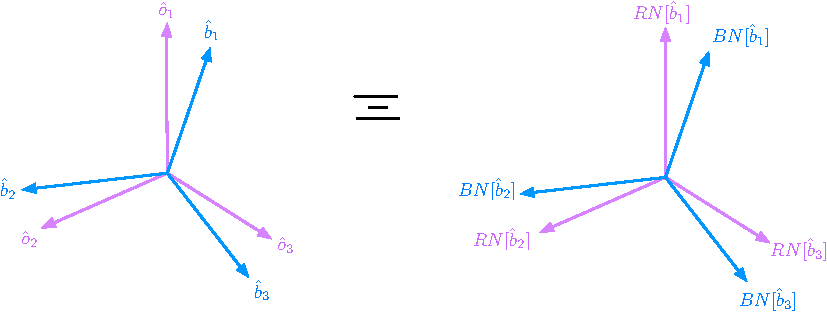
\includegraphics[width=7cm]{Figures/Fig2}
  }
  \caption{Illustration of the planet orbit frames, Hill $\mathcal{H}$ and Velocity $\mathcal{V}$.}
  \label{fig:Fig1}
\end{figure}
Figure~\ref{fig:Fig1} illustrates the relation between the Hill orbit frame $\mathcal{H}$ and the Velocity orbit frame.  $\mathcal{V}$. These two frames differ by a 3-axis rotation with the angle $-\beta$.  In terms of $\beta$, the DCM to map from $\mathcal{H}$ to $\mathcal{V}$ is given by
\begin{equation}
  \label{eq:VH1}
  [VH] = [M_{3}(-\beta)] = \begin{bmatrix}
    \cos\beta & -\sin\beta & 0 \\
    \sin\beta & \cos\beta &0 \\
    0 & 0 & 1
  \end{bmatrix}
\end{equation}
In terms of the classical set of orbital elements, this DCM can also be expressed as
\begin{equation}
  \label{eq:VH2}
  [VH] = \begin{bmatrix}
    \dfrac{1 + e \cos f}{\sqrt{1+e^{2}+2e \cos f}} & 
    -\dfrac{e \sin f}{\sqrt{1+e^{2}+2e \cos f} }
    & 0 \\
    \dfrac{e \sin f}{\sqrt{1+e^{2}+2e \cos f}}  & \dfrac{1 + e \cos f}{\sqrt{1+e^{2}+2e \cos f}} & 0\\
    0 & 0 & 1
  \end{bmatrix}
\end{equation}
\section{Introduction}
\begin{figure}[htb]
  \centerline{
  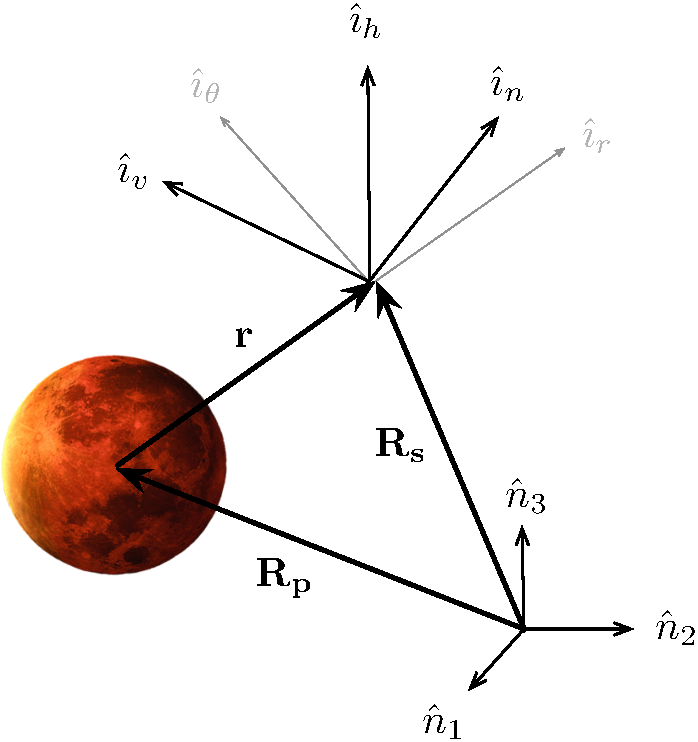
\includegraphics[width=7cm]{Figures/Fig3}
  }
  \caption{Illustration of the inertial frame $\mathcal{N}:\{ \hat{\bm n}_{1}, \hat{\bm n}_{2}, \hat{\bm n}_{3} \}$ and the orbit frames Hill $\mathcal{H}:\{ \hat{\bm\imath}_{r}, \hat{\bm\imath}_{\theta}, \hat{\bm\imath}_{h} \}$ and Velocity $\mathcal{V}:\{ \hat{\bm\imath}_{n}, \hat{\bm\imath}_{v}, \hat{\bm\imath}_{h} \}$ .}
  \label{fig:Fig2}
\end{figure}
In this module, a general axis is to be aligned with a principal Velocity frame axis and stay pointing fixedly on it. Note that the presented technique does not require the Velocity orbit frame $\mathcal{V}$ to coincide with the inertial frame $\mathcal{N}:\{ \hat{\bm n}_{1}, \hat{\bm n}_{2}, \hat{\bm n}_{3} \}$.\par 
Figure~\ref{fig:Fig2} illustrates the general situation in which $\bm{R}_{s}$ is the position vector of the spacecraft with respect to the inertial frame and $\bm{R_{p}}$ is the position vector of the orbited celestial body with respect to the inertial frame as well.
The relative position of the spacecraft with respect to the planet is obtained by simple substraction:
\begin{equation}
  \label{eq:r}
  \bm r = \bm R_{s} -  \bm R_{p}
\end{equation}
The same methodolgy is applied to compute the relative velocity vector:
\begin{equation}
  \label{eq:v}
  \bm v = \bm v_{s} -  \bm v_{p}
\end{equation}
Having $\bm r$ and $\bm v$, the Hill frame orientation is completely defined:
\begin{subequations}
  \begin{equation}
  \hat{\bm\imath}_{r} = \frac{\bm r}{r} 
  \end{equation}
  \begin{equation}
  \hat{\bm\imath}_{h} = \frac{\bm{r}\times{\bm{v}}}{r · v}
  \end{equation}
  \begin{equation}
  \hat{\bm\imath}_{\theta} = \hat{\bm\imath}_{h} \times \hat{\bm\imath}_{r}
  \end{equation}
\end{subequations}
\section{Velocity Frame Rate Development}
Next the Velocity frame rate $\dot\beta$ relative to the orbit frame is determined.
Note the following identities from ~\eqref{eq:VH1} and ~\eqref{eq:VH2}: 
\begin{equation}
  \label{eq:tanbeta}
  \tan\beta = \frac{e \sin f}{1 + e \cos f}
\end{equation}
\begin{equation}
  \label{eq:cos2beta}
  \cos^{2}\beta^{} = \frac{(1+e \cos f)^{2}}{1+e^{2}+2 e \cos f}
\end{equation}
Taking the derivative of Eq.~\eqref{eq:tanbeta} yields
\begin{equation}
  \label{eq:dbeta}
  \dot\beta =   \frac{ e (e+\cos f)}{1+e^{2}+2 e \cos f} \dot f
\end{equation}
To find the relative angular acceleration $\ddot\beta$, Eq.~\eqref{eq:dbeta} is differentiated again.
\begin{equation}
  \label{eq:ddbeta}
  \ddot\beta = 
   \frac{e(e+\cos f)}{1+e^{2}+2 e \cos f} \ddot f
   +\frac{
  e  (e^{2}-1)\sin f
  }{
  (1+e^{2}+2 e \cos f)^{2}
  } \dot f^{2}
\end{equation}
The true anomaly rate and acceleration are determined through the standard astrodynamics relations:
\begin{align}
  \dot f &= \frac{h}{r^{2}}
  \\
  \ddot f &= - 2 \frac{\bm v \cdot \hat{\bm\imath}_{r}}{r} \dot f
\end{align}
Following, let us evaluate the Velocity frame angular vectors.  As both the $\mathcal{V}$ and $\mathcal{H}$ frame rotate about the common $\hat{\bm\imath}_{h}$ axis, note that
\begin{equation}
  \label{eq:omegaVN}
  \bm\omega_{V/N} = \bm\omega_{V/H} + \bm\omega_{H/N} = (-\dot\beta + \dot f) \hat{\bm\imath}_{h}
\end{equation}
\begin{equation}
  \label{eq:domegaVN}
  \dot{\bm\omega}_{V/N} = \dot{\bm\omega}_{V/H} + \dot{\bm\omega}_{H/N} = (-\ddot\beta + \ddot f) \hat{\bm\imath}_{h}
\end{equation}

\section{Angular Velocity Descriptions}
Let $\mathcal{R}_{0}$ reference the Velocity orbit frame. Thus, $\bm\omega_{R_{0}/N}$ and $\dot{\bm\omega}_{R_{0}/N}$ correspond to the expressions in ~\eqref{eq:omegaVN} and ~\eqref{eq:domegaVN} respectively.
Let the sought general reference frame be $\mathcal{R}$. The attitude tracking control requires the angular rate $\bm\omega_{R/N}$ and acceleration $\dot{\bm\omega}_{R/N}$. 
Since the pointing towards the orbit axis is constant, the desired reference $\mathcal{R}$ does not move relative to $\mathcal{R}_{0}$. Thus, the angular velocity of the reference frame happens to be
\begin{equation}
  \label{eq:omega_R}
  \bm\omega_{R/N} = \bm\omega_{R/R_{0}} - \bm\omega_{R_{0}/N} = \bm\omega_{R_{0}/N} = \frac{1+e \cos f}{1+e^{2} + 2 e \cos f} \dot f \hat{\bm\imath}_{h}
\end{equation}
where $\dot\beta$ and $\dot f$ have been substituted by their correspinding expressions.\newline
Similarly, we find
\begin{equation}
  \label{eq:domega_R}
  \dot{\bm\omega}_{R/N} = \dot{\bm\omega}_{R/R_{0}} + \dot{\bm\omega}_{R_{0}/N} = \dot{\bm\omega}_{R_{0}/N} =
  \left( \frac{1+e\cos f}{1+e^{2}+2 e \cos f} \ddot f
  - \frac{
  e  (e^{2}-1)\sin f
  }{
  (1+e^{2}+2 e \cos f)^{2}
  } \dot f^{2} \right) \hat{\bm\imath}_{h}
\end{equation}
where $\ddot\beta$ and $\ddot f$ have been substituted by their correspinding expressions.

\bibliographystyle{unsrt}
\bibliography{references}

\end{document}
